\setchapterpreamble[u]{\margintoc}
\chapter{Conclusiones}
\labch{conclusions_spanish}
\label{sec:conclusions_spanish}

En esta tesis se han propuesto soluciones para registrar imágenes \acrshort{rgb}, multiespectrales y térmica, con el objetivo de alcanzar un sistema compuesto por múltiples capas de información. Después, se extendió este enfoque al 3D mediante la proyección de la información registradas en nubes de puntos \acrshort{rgb} con una densidad muy elevada. También se ha logrado proyectar información hiperespectral en una nube de puntos 2.5D. Además, el hipercubo generado se comprimió y renderizó en tiempo real utilizando una estructura basada en \textit{stacks}. A continuación se simuló un sensor \acrshort{lidar} como alternativa a la captura de datos reales, evitando así el coste de adquisición del sensor y las posteriores tareas de procesamiento, limpieza y anotación de datos capturados. Este simulador permitió obtener conjuntos de datos muy grandes, tanto de \acrshort{lidar} aéreo como terrestre, con anotaciones semánticas e intensidad. Tanto el simulador como los procesos de fusión se han implementado en la \acrshort{gpu}, obteniendo una mejora notable de rendimiento en comparación con otras soluciones comerciales. Por último, tanto los datos reales como simulador se han aplicado a múltiples casos de estudio, desde optimización de escaneos \acrshort{lidar}, a la identificación de anomalías térmicas y la clasificación de variedades de vid en imágenes hiperespectrales. 

% En esta tesis se ha llevado a cabo la fusión de múltiples fuentes de datos obtenidas mediante teledetección, donde cada una de ellas se centra en un intervalo de longitudes de onda diferentes. El algorithmo de \textit{Enhanced Correlation Coefficient}, o \acrshort{ecc} \cite{evangelidis_parametric_2008}, se ha utilizado para llevar a cabo el registro de imágenes con unas diferencias bastante notables de intensidad. A pesar de estas diferencias, se obtuvo una mejora considerable en la correlación de imágenes \acrshort{rgb}, multiespectrales e infrarrojas tras ser alineadas.También se evaluó si era posible hacer este proceso más eficiente 1) disminuyendo el tamaño de imagen, y 2) eliminando detalles mediante transformaciones de desenfoque. Se mostró que el desenfoque contribuía a reducir significativamente el tiempo de respuesta, mientras que la correlación se mantenía en valores muy similares a los obtenidos sin aplicar ambas operaciones, 1) y 2).

% A partir de aquí disponemos de un sistema compuesto por múltiples capas de información en el espacio de la imagen. El siguiente paso es la proyección de este sistema en productos de mayor dimensionalidad, como una nube de puntos 3D. Para ello, se reconstruyeron nubes de puntos \acrshort{rgb} muy densas mediante fotogrametría, y utilizando este resultado, se proyectaron los puntos 3D en el espacio de la imagen para introducir el sistema multi-capa en nubes de puntos. Los resultados de esta metodología eran mucho más precisos a nivel geométrico y presentaban mayor densidad de puntos, en comparación con las nubes obtenidas empleando fotogrametría. Además, la implementación se llevó a cabo en la \acrshort{gpu}, por lo que nuestro método también era mucho más rápido. Durante este proceso se tuvo en cuenta la oclusión mediante el uso de \textit{$z$-buffers}, e igualmente, se acumularon los valores proyectados en un punto 3D mediante funciones de agregación y funciones penalty, con el fin de minimizar la disimilitud. 

% En el caso de las imágenes hiperespectrales, la metodología propuesta es bastante diferente de la anterior. Primero fue necesario corregir las distorsiones geométricas, utilizando un ortomosaico \acrshort{rgb} como referencia. Una vez corregidas se generó un ortomosaico hiperespectral que sería proyectado posteriormente en una nube de puntos voxelizada. El hipercubo resultante presentaba un consumo bastante significativo de memoria, y para mitigar este problema se comprimió en la dimensión radiométrica utilizando un enfoque basado en \textit{stacks} \cite{graciano_quadstack_2021}. Esto a su vez presentaba desventajas en el renderizado, dado que era necesario iterar por cada píxel dentro de un \textit{shader}. La solución planteada consistía en construir un frame de manera iterativa, de tal modo que éste se completa en unos pocos frames, en lugar de renderizarse por completo en cada nuevo frame. 
% This dissertation has addressed the fusion of remotely sensed data acquired by multiple devices that comprise different spectra intervals. The Enhanced Correlation Coefficient (\acrshort{ecc}) was first proposed to solve the image-matching of images with notable radiometric differences. Once a multi-layer system was achieved in the image space, this data stack was projected into products of larger dimensionality. To this end, \acrshort{rgb} point clouds with high \acrshort{lod} were reconstructed with photogrammetry, and from here, points were projected back to the image where the data stack was achieved. This pipeline was proven to generate much more precise and dense 3D point clouds than those achieved with photogrammetry. In addition, the projection of multispectral and infrared data was fastened using \acrshort{gpgpu}, thus achieving a notable performance improvement. Occlusion was handled with $z$-buffers, and the aggregation of multiple image samples in 3D points was optimized with aggregation and penalty functions. On the other hand, hyperspectral swaths were fused with visible point clouds with a different pipeline that suits better the conditions on which this data is acquired. The geometrical distortions were achieved by matching swaths with an \acrshort{rgb} orthomosaic, and then, a hyperspectral orthomosaic was composed and projected into a voxelized point cloud. The large footprint of these data was reduced by compressing it, and the shortcomings derived from it in the rendering were tackled by iteratively constructing a frame.

% The tedious task of acquiring, processing and including additional data in real-world datasets was partially avoided by generating synthetic \acrshort{lidar} data. Static and procedural scenarios were indexed in a \acrshort{bvh} for rapidly solving spatial intersections, and besides that, the simulation was solved with \acrshort{gpgpu}. Together with procedural modelling, this tool helps to generate large training datasets for \acrshort{ai}. Airborne and terrestrial scans were introduced, including the definition of paths to be followed. This virtual sensor was not only aimed at solving intersections but also frequent \acrshort{lidar} errors were simulated. Then, the estimation of \acrshort{lidar} intensity was addressed with two different approaches, based on analytical \acrshort{brdf}s and collected \acrshort{brdf} databases. The latter was proven to be much easier to integrate and is considerably more efficient at the expense of storing a minimal part of the database in the \acrshort{gpu}.

% En este trabajo se han propuesto múltiples metodologías para fusionar la información adquirida por diferentes sensores integrados en un dron. El método de registro de imágenes conocido como "Enhanced Correlation Coefficient" (\acrshort{ecc}), propuesto por Evangelidis y Psarakis \cite{evangelidis_parametric_2008}, se ha utilizado como base para alcanzar un sistema compuesto por múltiples capas de información. Dicho algoritmo no se había explorado aún en teledetección para registrar imágenes con observaciones radiométricas muy diferentes. En esta tesis, se ha mostrado la eficacia de dicho método para fusionar información en el espectro visible e infrarrojo. A partir de aquí, este sistema multicapa se ha extendido a nubes de puntos 3D mucho más fáciles de interpretar y visualizar por operadores humanos. La reconstrucción de nubes 3D suele llevarse a cabo mediante fotogrametría; no obstante, ésta es bastante proclive a introducir errores geométricos con imágenes de resolución reducida, como las imágenes térmicas y multiespectrales. Además, una resolución tan reducida también deriva en una baja densidad de puntos. Una vez descritos estos inconvenientes, se propone estimar con fotogrametría una nube de puntos de referencia utilizando únicamente imágenes de alta resolución, mientras que el resto de la información se proyecta en dicha nube de puntos. Por tanto, el sistema compuesto por múltiples capas se extiende al 3D. Por otro lado, los hipercubos también se han proyectado sobre nubes de puntos 3D, aunque son muy pocos los trabajos que se enfocan en esta tarea en la literatura. En este caso, el proceso de adquisición de datos es significativamente más peculiar, dado que el sensor funciona escaneando líneas espaciales a lo largo de una distancia considerable. Por tanto, son muy pocas las imágenes obtenidas, y éstas presentan grandes dimensiones. Por tanto, dadas estas peculiaridades, entre las que se incluye un ángulo de visión \textit{nadir}, la extensión al 3D no es tal sino simplemente un mapa de altura en 2.5D. 

% Por otro lado, los datos obtenidos mediante sensores reales presentan algunas desventajas, tales como la lentitud del proceso de adquisición así como en las tareas de procesamiento (eliminación de ruido, etiquetado, etc.), además del elevado que presentan tecnologías como el \acrshort{lidar}. Para evitar algunas de estas desventajas, se implementó un simulador \acrshort{lidar} con el fin de obtener conjuntos de datos sintéticos que podrían incluir cualquier tipo de información en cada punto generado. A día de hoy, se ha explorado la generación de imágenes sintéticas mediante Redes Generativas Adversarias (\acrshort{gan}), aunque debido al ámbito limitado de esta tesis, se ha introducido únicamente la simulación de un sensor \acrshort{lidar}. Dicho simulador se ha empleado para construir grandes conjuntos de datos tanto de misiones aéreas como terrestres. Sobre cada punto se evaluó la estimación de información radiométrica utilizando dos enfoques diferentes. Ambos fueron capaces de producir nubes de puntos con valores de intensidad, mostrando diferencias muy notables entre superficies modeladas con materiales distintos. 

% Finalmente, los resultados obtenidos se han empleado en diversas aplicaciones. En primer lugar, la simulación \acrshort{lidar} se aplicó a la optimización de escaneos utilizando metaheurísticas que ayudaron tanto a reducir el número de posiciones como a calcular las posiciones óptimas dentro de un espacio tridimensional. También, las imágenes y nubes de puntos térmicas se han utilizado en la identificación de restos arqueológicos, y por último, las imágenes hiperespectrales se han procesado para su posterior clasificación en diferentes variedades de vid utilizando Deep Learning.

A nivel personal, estos tres últimos años me han ayudado a mejorar como investigador. El trabajo realizado ha dado lugar a importantes resultados que han sido publicados en revistas y congresos de primer nivel en el campo de la teledetección, mientras que otros están aún en proceso de revisión. Además, he tenido el placer de participar en trabajos de otros compañeros, que, a pesar de no formar parte de la temática de esta tesis, han contribuido enormemente a aprender mucho más acerca de la informática gráfica.

\section{Resumen de las contribuciones presentadas}

En primer lugar, se propuso una metodología para \textbf{corregir y fusionar imágenes procedentes de múltiples sensores}. El algoritmo de registro de imágenes \acrshort{ecc} se utilizó para poder registrar información obtenida en longitudes de onda muy diferentes. Se obtuvieron buenos resultados a pesar de las diferencias radiométricas tan significativas, y se aplicó en la fusión de imágenes visibles, multiespectrales y térmicas. Además, la eficacia de dicho algoritmo se evaluó mediante la correlación obtenida en el registro de imágenes con un tamaño menor y sobre las que se aplicaron operaciones de desenfoque. De estos últimos experimentos se concluye que tanto el desenfoque aplicado como la reducción de tamaño permiten reducir considerablemente el tiempo de respuesta mientras que se obtiene una correlación similar.

La metodología de registro de imágenes representa la base de los primeros capítulos de esta tesis. El siguiente paso es la \textbf{proyección de las imágenes registradas en nubes de puntos 3D}. Trabajar con nubes de puntos es mucho más intuitivo para visualizar e identificar objetos en una escena. Sin embargo, éstas deben reunir ciertas condiciones, como ser lo suficientemente densas o presentar una geometría sin errores en la reconstrucción. Por tanto, se ha definido una metodología para la generación de nubes de puntos con información \acrshort{rgb}, térmica y multiespectral. En primer lugar, se reconstruye una nube de puntos \acrshort{rgb} precisa y de alta densidad mediante fotogrametría, y a continuación, el resto de conjuntos de datos se proyecta sobre esta nube de puntos que garantiza unas condiciones óptimas (tanto en geometría como en densidad de puntos). De este modo, se evitan algunos de los principales inconvenientes de la fotogrametría en imágenes de baja resolución, como térmicas y multiespectrales. Además, se comparó nuestra solución con software comercial, evidenciando una mejora bastante notable en términos de 1) tiempo de respuesta, 2) densidad y 3) tamaño. Otros factores que se tuvieron en cuenta fueron la proyección de información teniendo en cuenta la oclusión mediante el uso de $z$-buffer, o la optimización de la agregación de valores procedentes de imágenes diferentes mediante el uso de funciones de agregación y funciones \textit{penalty}. Con este último enfoque se consigue que los valores agregados minimicen la disimilitud de dicho valor respecto de las muestras iniciales. 

Además, esta metodología se implementó en la \textbf{\acrshort{gpu}} para equiparla a soluciones comerciales como Agisoft Metashape o Pix4Dmapper. Se obtuvo un tiempo de respuesta mucho menor que el observado en estas soluciones comerciales. También se comprobaron otras mejoras, como la reordenación global y local de la nube de puntos. Los experimentos llevados a cabo mostraron que la reordenación global mejoraba significativamente el tiempo de respuesta, a pesar de incluir el tiempo derivado de la ordenación. Por otro lado, la ordenación local no obtuvo mejores resultados en nubes de puntos de mayor tamaño debido a la sobrecarga derivada de ordenar globalmente y después reordenar aleatoriamente grupos muy pequeños. Se concluye, por tanto, que este último enfoque podría ser más viable para procesos que se ejecutan más de una vez, y por tanto, sólo ordenan la información una vez.

El siguiente paso es la generación de \textbf{nubes de puntos hiperespectrales}, que, hasta donde sabemos, no se había logrado anteriormente, al menos fuera de un laboratorio. Para ello, las imágenes hiperespectrales se corrigieron utilizando como referencia un ortomosaico \acrshort{rgb}, y después, se construyó un ortomosaico hiperespectral utlilizando la optimización previamente resuelta con funciones de agregación y funciones \textit{penalty}. Posteriormente, la información hiperespectral se proyectó sobre una nube de puntos 2.5D cuyo tamaño de vóxel se corresponde con el \acrshort{gsd} de las imágenes hiperespectrales. Debido al gran tamaño del hipercubo resultante, éste se comprimió en la dimensión radiométrica siguiendo un enfoque basado en \textit{stacks}. No obstante, esta compresión también dificultó la visualización en tiempo real dado que requería múltiples iteraciones por cada píxel en un \textit{shader}. Este inconveniente se mitigó construyendo las imágenes en múltiples fotogramas. Al igual que soluciones previas, todo esta metodología se desarrollado en la \textit{gpu}, presentando por tanto una notable mejora en el tiempo de respuesta.

A continuación, se describió un \textbf{simulador \acrshort{lidar}} con el objetivo de evitar tareas tan tediosas de la adquisición, limpieza, procesamiento o etiquetado de datos. Dicho simulador permite resolver intersecciones de rayos y geometría en un tiempo de respuesta muy reducido, además de introducir errores sistemáticos y aleatorios descritos en la literatura. Estos errores se derivan de partículas atmosféricas, materiales con una reflectancia elevada, o bien se corresponden con la distancia de escaneo o la inclinación de la superficie intersectada. La simulación se ha parametrizado para integrar un amplio número de sensores \acrshort{lidar} comerciales. Además, otro factor clave es la generación de escenarios procedurales que permiten obtener un gran número de escenas (y nubes de puntos) diferentes. Los modelos que conforman estas escenas se asocian con materiales y etiquetas semánticas a través de una especificación basada en el nombre de los modelos. Esta tarea sólo se lleva a cabo una vez para escenarios procedurales, y por tanto, es mucho más eficiente. Posteriormente, se ha establecido una comparativa entre dos métodos diseñados para la estimación de intensidad \acrshort{lidar}. Primero, se resolvió este problema con \acrshort{brdf}s analíticas, como en un sombreado tradicional, y posteriormente se utilizaron \acrshort{brdf}s procedentes de bases de datos recientementes que obtienen los datos de un goniofotómetro. La comparativa evidenció que el segundo método presentaba un mayor consumo de memoria, pero también era más eficiente y estaba basado en datos reales. En cualquier caso, se redujo su consumo de memoria al máximo asumiendo que tanto el emisor como el receptor del \acrshort{lidar} ocupaban la misma posición. Todo el proceso de simulación \acrshort{lidar} se implementó en la \acrshort{gpu} para resolver de manera eficiente escaneos aéreos y terrestres, desde la etapa de generación de pulsos \acrshort{lidar} hasta la propia resolución de colisiones.

A diferencia de los simuladores \acrshort{lidar} previamente descritos en la literatura, nuestra solución permite llevar a cabo \textbf{escaneos tanto terrestres como aéreos}. El primer tipo de simulación es el más habitual, mientras que el segundo apenas se ha descrito con anterioridad. Ambos requieren una trayectoria definida por el usuario o calculada automáticamente, mientras que las misiones aéreas también emplean diferentes patrones de escaneo, entre los que se incluyen el barrido en paralelo, en zigzag y elipsoidal. También se simulan múltiples retornos, los cuales permiten mostrar cómo se eliminan intersecciones de árboles y vegetación para obtener los puntos pertenecientes al suelo, y un \acrshort{lidar} batimétrico que permite alcanzar superficies debajo del agua. 

Finalmente, los conjuntos de datos y resultados obtenidos en capítulos anteriores se han empleado en diversos casos prácticos. En primer lugar, se utilizó la simulación \acrshort{lidar} para diseñar un \textbf{plan de escaneo} en edificios, minimizando y optimizando las posiciones necesarias en función de la oclusión de la escena y la calidad de los retornos simulados. Este problema se resolvió mediante metaheurísticas guiadas por funciones objetivo en las que no interviene el usuario, y por tanto, se integraron fácilmente en la simulación de la que ya disponíamos. Después se han utilizado \textbf{imágenes y nubes de puntos térmicas para inspeccionar un yacimiento arqueológico}, donde se detectaron zonas anómalas que podrían corresponderse con restos aún no explorados. Por último, se han procesado y corregido imágenes hiperespectrales para la posterior \textbf{clasificación de variedades de vid}. Las técnicas tradicionales, basadas en la correlación del perfil espectral, no son apropiadas para la clasificación de materiales cuyos perfiles espectrales son muy similares. En su lugar, se emplearon redes neuronales con capas descritas en el estado del arte, como las capas de atención espacial. Los hipercubos se han dividido en pequeños bloques, con un tamaño que se ha ajustado durante la experimentación, y se han reducido a una sola etiqueta. Por tanto, la clasificación de cada muestra depende también de su vecindario. No sólo se ha comprobado la red propuesta sobre datos de dron, a pesar de constituir el objetivo principal, sino también sobre datos de satélite, obteniendo una precisión muy alta en ambos casos. 

\section{Trabajo futuro}

La teledetección y la inteligencia artificial se encuentran en constante evolución, y a pesar de ello, existen algunos trabajos futuros que debieran explorarse a partir de esta tesis:
\begin{itemize}
    \item El registro de imágenes se llevó a cabo utilizando hardware que no estaba orientado a altas prestaciones, y por lo tanto, se exploraron alternativas para mejor la eficiencia como la reducción de tamaño de imágenes o su desenfoque. No obstante, otra alternativa consiste en explorar un esquema piramidal que, partiendo de un tamaño muy reducido, permita obtener una transformación inicial con menor nivel de detalle (pero capaz de identificar grandes cambios). Este esquema se muestra en la Figura \ref{fig:image_pyramid_spanish}. A medida que se incrementa el tamaño de imagen, el nivel de detalle del registro es mayor, pero los cambios son de menor entidad, y por tanto, se estiman en un menor tiempo de respuesta. Además de reducir la latencia, este enfoque también podría ayudar a registrar imágenes con diferencias mucho mayores.
    \begin{figure}
        \centering
        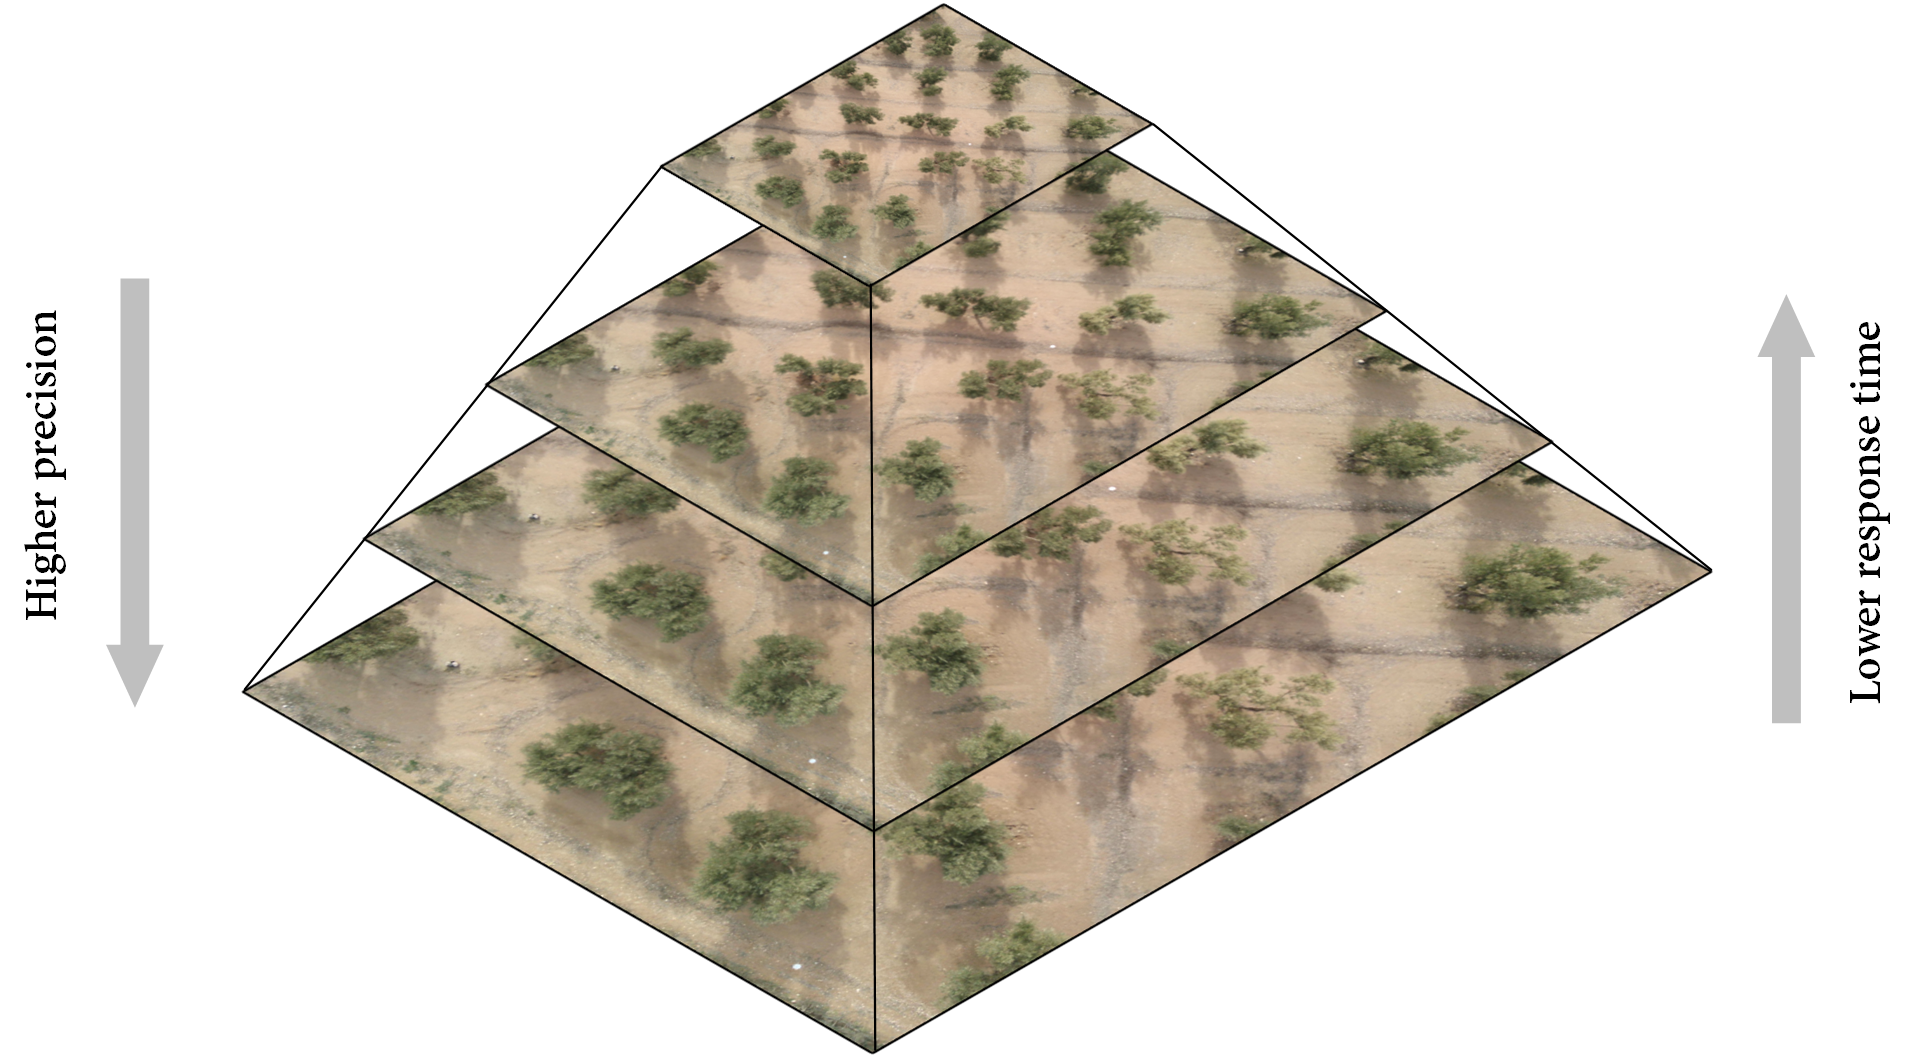
\includegraphics[width=\linewidth]{figs/conclusions/image_pyramid.png}
        \caption{Registro de imagen iterativo, donde un mayor tamaño de imagen implica mayor tiempo de respuesta y mayor precisión en la estimación de la matriz de transformación.}
        \label{fig:image_pyramid_spanish}
    \end{figure}
    \item El registro de imágenes formaba parte de la fase de lectura y procesamiento de datos en las comparaciones establecidas con software de fotogrametría. Por lo tanto, esta etapa podría acelerarse aún más implementando \acrshort{ecc} en la \acrshort{gpu}.
    \item La generación de nubes de puntos 3D con una densidad de puntos muy elevada, con información \acrshort{rgb}, térmica y multiespectral; sin embargo, las nubes de puntos con una dimensionalidad tan elevada son también más difíciles de renderizar en tiempo real. Aunque el renderizado utilizando \textit{compute shaders} ayudó considerablemente a reducir a la latencia \cite{schutz_rendering_2021}, podría mejorarse aún más con diferentes niveles de detalle (\acrshort{lod}) \cite{schutz_gpu-accelerated_2023}. Del mismo modo, podría ayudar a renderizar hipercubos comprimidos, dado que uno de los principales inconvenientes encontrados fue un renderizado mucho menos eficiente que de costumbre.
    \item La compresión de hipercubos se implementó reduciendo la resolución radiométrica mediante una representación basada en pilas, mientras que la compresión espacial no obtuvo buenos resultados debido a la gran variabilidad de los datos en la dimensión espacial. En lugar de una representación basada en pilas, la compresión podría llevarse a cabo en la dimensión espacial, de mucho mayor tamaño que la dimensión espectral. 
    \item La optimización \acrshort{lidar} se exploró en la identificación de ubicaciones óptimas para el escaneo con \acrshort{lidar} terrestre. Sin embargo, hay otros tipos de tecnología \acrshort{lidar} que podrían explorarse, especialmente aquellos que requieren una trayectoria. De esta manera, las optimizaciones basadas en poblaciones podrían ser de gran utilidad para el cálculo de rutas \cite{roberge_fast_2018}. La optimización de \acrshort{lidar} aéreo también podría explorarse para determinar cuál es la configuración óptima para escanear una escena específica con una densidad elevada, partiendo por ejemplo de un \acrshort{dsm}.
    \item Una línea similar consiste en evaluar misiones de dron calculando una trayectoria que garantice ciertos requisitos de solapamiento y cobertura en función del tiempo, la altitud y la velocidad de vuelo, entre otros factores. Este mismo problema se ha estudiado para misiones de dron genéricas \cite{pessacg_simplifying_2022}; no obstante, podría mejorarse aún más en función de la geometría de la escena, representada mediante modelos rápidamente esbozados. Esto podría ser de especial interés para vuelos que requieren observaciones oblicuas, con un ángulo configurable por el usuario. 
    \item Hasta ahora, las simulaciones \acrshort{lidar} se han utilizado para generar grandes conjuntos de datos ya etiquetados. Sin embargo, los conjuntos de datos generados deben comprobarse en tareas de clasificación y segmentación mediante Deep Learning, con el fin de verificar que los conjuntos de datos de entrada podría sustituirse, al menos de manera parcial, por datos sintéticos. Nótese que algunos de los errores simulados se omiten durante la voxelización de  una nube de puntos \cite{hackel_semantic3d_2017, behley_towards_2021}. Por tanto, es necesario comprobar si los conjuntos de datos generados pueden realmente sustituir, al menos parcialmente, a conjuntos de datos reales. 
    \item Además de \acrshort{lidar}, hay otros sensores basados en imágenes que pueden ser simulados mediante redes generativas adversarias (Generative Adversarial Networks) como la que se muestra en la Figura \ref{fig:conclusiones_gan}. Éstas permiten generar conjuntos de datos no supervisados que permitirían, por ejemplo, construir imágenes térmicas a partir de imágenes visibles con el fin de ampliar conjuntos de datos. Los trabajos ya existente no han conseguido resolver este problema utilizando únicamente información visible como entrada \cite{li_multi-branch_2019, li_i-gans_2021, kniaz_thermalgan_2019, ozkanoglu_infragan_2022, yi_cycle_2023}. Sin embargo, esta tarea podría ayudarse de anotaciones semánticas que permitan identificar superficies distintas, las cuales a su vez se relacionan con diferente información radiométrica.
    \begin{figure}[ht]
        \centering
        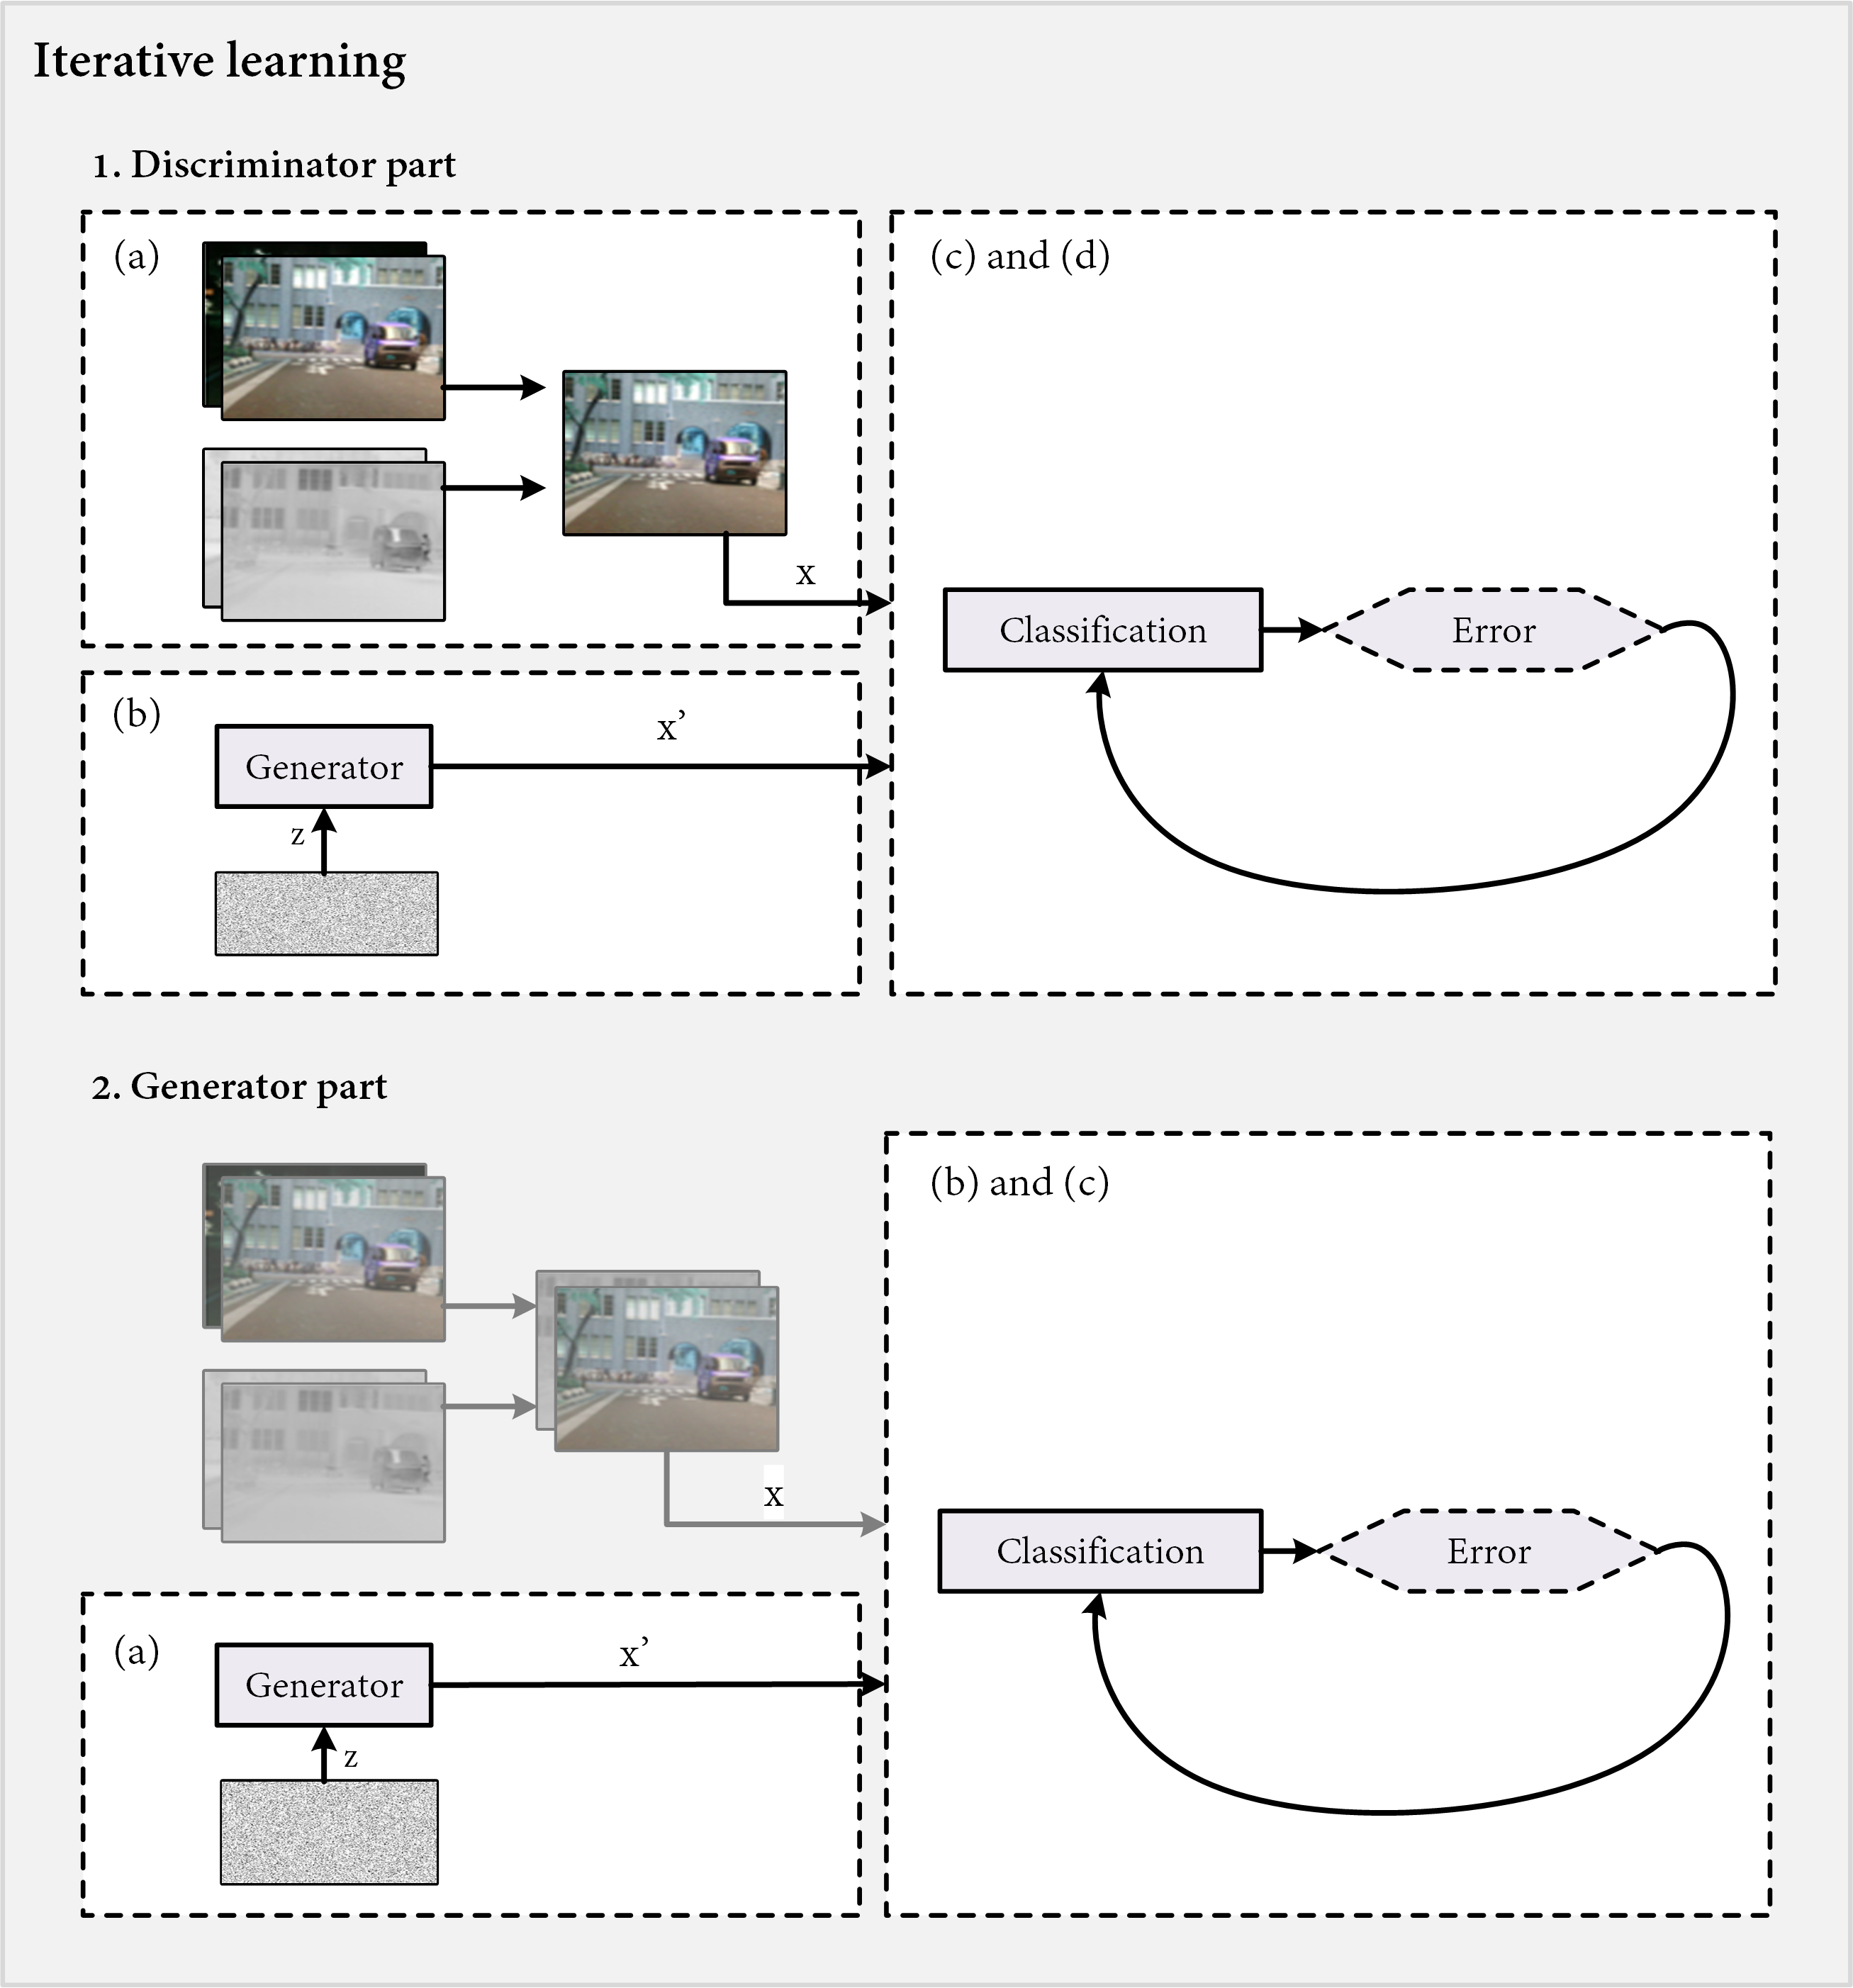
\includegraphics[width=\linewidth]{figs/conclusions/gan.png}
        \caption{Esquema de una red generativa adversaria, compuesta a su vez por dos modelos diferentes: generador y discriminador. El primero se entrena para producir datos realistas, mientras el segundo debe discernir, con la mayor eficacia posible, si los datos de entrada son reales o no.}
        \label{fig:conclusiones_gan}
    \end{figure}
    \item La clasificación de variedades de vid se resolvió con Deep Learning; sin embargo, este modelo podría mejorarse integrando más variedades y recopilando más conjuntos de datos en diferentes etapas del año. Además, existen otros enfoques interesantes para abordar esta misma tarea, desde la clasificación multi-instancia \cite{meerdink_multitarget_2022} hasta el aprendizaje por comparación \cite{guan_spatial-spectral_2022}. 
\end{itemize}
